% Laboratory Manual For Wildlife Forensics

\documentclass[12pt, hidelinks]{article}

%-- Activate below to make default font sans serif --%
%\renewcommand{\familydefault}{\sfdefault}

%-- Set Margins --%
\usepackage[margin=2.5cm]{geometry}

%-- Package for text colouration --%
\usepackage[usenames,dvipsnames]{color} 

%-- Package for Links --%
\usepackage{hyperref} 

%-- Set paragraph spacing and indentation --%
\setlength{\parindent}{0pt}
\setlength{\parskip}{0.5cm}

%-- Package for controlling spacing of lists --%
\usepackage[shortlabels]{enumitem}
\setlist[enumerate]{topsep=-5pt}
\setlist[itemize]{topsep=-5pt}

%-- Package and settings for making caption width less than page width --%
\usepackage[margin=2cm]{caption}


%-- Package and settings for reducing space after section titles
\usepackage{titlesec}
\titlespacing\section{0pt}{12pt plus 4pt minus 2pt}{-10pt plus 2pt minus 2pt}
\titlespacing\subsection{0pt}{12pt plus 4pt minus 2pt}{-10pt plus 2pt minus 2pt}
\titlespacing\subsubsection{0pt}{12pt plus 4pt minus 2pt}{0pt plus 2pt minus 2pt}


%--------------------------------%
%     Custom Colours             %
%--------------------------------%
\usepackage[table]{xcolor}
\definecolor{myblue}{rgb}{0,0.3,0.6}
\definecolor{myblue2}{rgb}{0,0.4,0.8}


%-- Packages for making nice tables --%
\usepackage{booktabs}
\usepackage{makecell}  % Required for specifying multiple rows within a table cell

%-- Packages for Proper Handling of Figures --%
\usepackage{graphicx}
\usepackage{float}


%---------------------------------------------------------------------------------------
\begin{document}

%-------------------------%
%  Title Page             %
%-------------------------%
\vspace*{2cm}

	\begin{center}
		\LARGE{\textbf{Wildlife Forensics:\\
		\vspace{0.5cm}
		 Laboratory Manual}}\normalsize{}\\
		
		\vspace{2cm}
		by\\
		Tim Frasier\\
		
		\vspace{2cm}
		
		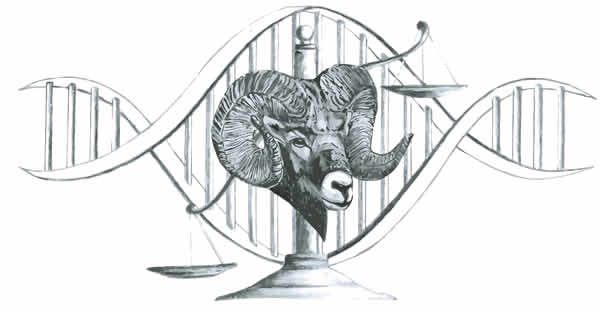
\includegraphics[width=0.5\textwidth]{figures/swfs.jpg}
	\end{center}


\newpage
%-------------------------%
%  Laboratory #1          %
%-------------------------%
\section{Laboratory \#1: Sample Collection}


	%------------------------%
	% Overview               %
	%------------------------%
	\subsection{Overview}
	Today we will discuss sample collection procedures for the class. Briefly, for this course we will be collecting food from local restaurants and performing genetic species identification of those samples to determine if the food was labelled correctly. Students will need to collect these samples during the following week so that the samples are ready for DNA extraction in Lab \#2.

 	As a class, we will decide what types of food to sample (fish, poultry, beef, etc.), and decide on a general sampling strategy.
	
	We will also discuss proper use of lab books, as well as the ingredients of lysis buffer, and the role of each ingredient in the solution.
	
	
	%------------------------%
	% Readings               %
	%------------------------%
	\subsection{Readings}
	The following readings are available on Brightspace, and should be read \emph{before} coming to lab.
		\begin{enumerate}
			\item Lee (2003)
			\item Hunter \& Hughey (2007)
		\end{enumerate}
	
	
	%------------------------%
	% Safety                 %
	%------------------------%
	\subsection{Safety}
	We will just be talking today, and therefore there are no personal protective equipment (PPE) requirements.
	
	
	%------------------------%
	% Supplies Needed        %
	%------------------------%
	\subsection{Supplies Needed}
	None.


\newpage
%-------------------------%
%  Laboratory #2          %
%-------------------------%
\section{Laboratory \#2: DNA Extraction}


	%------------------------%
	% Overview               %
	%------------------------%
	\subsection{Overview}
	In today's lab we will extract DNA from the samples that were previously collected.
	
	
	%------------------------%
	% Safety                 %
	%------------------------%
	\subsection{Safety}
	For laboratory work today, we will be using the reagents included in the QIagen DNeasy Blood \& Tissue Kit. None of these reagents are particularly harmful. However, there are still some requirements:
	
	\underline{Required Personal Protective Equipment (PPE):}
		\begin{enumerate}
			\item Close-toed shoes
			\item Long pants
			\item Lab coats
			\item Goggles
			\item Gloves
		\end{enumerate}
	
	
	%------------------------%
	% Supplies Needed        %
	%------------------------%
	\subsection{Supplies Needed}
		\begin{enumerate}
			\item Qiagen DNeasy Blood \& Tissue Kit (for at least 40 samples)
			\item 95\% Ethanol ($\sim$25 ml)
			\item Benchtop centrifuges ($\times$2)
			\item Pipettes
				\begin{enumerate}
					\item 10--100 $\mu$l: $\times$ 6
					\item 100--1,000 $\mu$l: $\times$ 6
				\end{enumerate}
			\item Tips: 3 tip boxes for each pipette size above
			\item Containers for tip waste
			\item Tubes
				\begin{enumerate}
					\item 1.5 ml: $\sim$80
					\item 0.6 ml: $\sim$80
				\end{enumerate}	
			\item Gloves (small, medium, and large)	
		\end{enumerate}
	
	
	%------------------------------%
	% Protocol                     %
	%------------------------------%
	\subsection{Protocol}	
		\begin{enumerate}
			\item Pipette 250 $\mu$l of each sample into a new 1.5 mL tube and label
			\item Add 250 $\mu$l of \textbf{AL Buffer} to each sample and mix well
			\item Add 250 $\mu$l of \textbf{95\% Ethanol} to each sample and mix well
			\item Transfer samples (750 $\mu$l) to spin columns and spin @ 7,500 $\times$ g for 1 minute
			\item Discard the collection tubes and replace with new ones
			\item Add 500 $\mu$l of \textbf{Buffer AW1} and spin @ 7,500 $\times$ g for minute
			\item Discard the collection tubes and replace with new ones
			\item Add 500 $\mu$l of \textbf{Buffer AW2} and spin @ 14,000 $\times$ g for 3 minutes
			\item Discard collection tubes and replace with new ones
			\item Spin samples again @ 14,000 $\times$ g for 1 minute
			\item Discard collection tubes and replace with 1.5 mL tubes
			\item Add 50 $\mu$l of \textbf{Buffer EB} to each sample, and let sit for 1 minute with the lids open
			\item Spin samples @ 7,500 $\times$ g for 1 minute
			\item Transfer DNA to 0.6 mL tubes and label
		\end{enumerate}


\newpage
%-------------------------%
%  Laboratory #3          %
%-------------------------%
\section{Laboratory \#3: Assessing DNA Quantity and Quality}	

	%------------------------------%
	% Overview                     %
	%------------------------------%
	\subsection{Overview}
	Today we will assess the quantity and quality of the DNA obtained from the extraction process. Quantity will be estimated based on spectrophotometry using a NanoDrop 2000 (ThermoFisher). DNA quality will be assessed by running $\sim$25 ng of DNA on a 1.5\% agarose gel, stained with GelRed and illuminated with UV light. DNA quality will be assessed based on the amount of smearing observed. The brightness of the band, relative to the Low Mass DNA Ladder standard, will also be used double-check the quantity estimates from the NanoDrop.


	%------------------------------%
	% Safety                       %
	%------------------------------%
	\subsection{Safety}
		\begin{itemize}
			\item UV light causes serious damage to your skin and your eyes!!!  NEVER look at a gel under UV light without proper eye protection. Always view gels through the ``viewer'' on the Gel Dock box, and ensure that the UV lights are off whenever the light box is not covered.
		\end{itemize}

	\underline{Required Personal Protective Equipment (PPE)}:
		\begin{enumerate}
			\item Closed-toed shoes
			\item Long pants
			\item Lab coats
			\item Gloves
			\item Goggles
		\end{enumerate}	


	%------------------------------%
	% Supplies Needed              %
	%------------------------------%
	\subsection{Supplies Needed}
		\begin{enumerate}
			\item Pipettes
				\begin{enumerate}
					\item 0.5--10 $\mu$l: $\times$ 6
				\end{enumerate}
			\item Tips: 4 tip boxes for each pipette size above	
			\item Containers for tip waste
			\item Tubes
				\begin{enumerate}
					\item 0.6 mL: $\sim$60
				\end{enumerate}	
			\item Gloves (small, medium, and large)
			\item Agarose (Tim will provide)
			\item 0.5X TBE Buffer (Tim will provide)
			\item TE$_{0.1}$ (Tim will provide)
			\item Orange G loading dye (Tim will provide)
			\item Low Mass DNA Ladder (Tim will provide) 
		\end{enumerate}


	%---------------------------------%
	% Estimating DNA Quantity         %
	%---------------------------------%
	\subsection{Estimating DNA Quantity}	
	We will estimate DNA quantity using a NanoDrop 2000, which is based on spectrophotometry.

		\begin{enumerate}
			\item Thaw your sample and mix well
			\item Evaluate standard samples to ensure that NanoDrop is functioning properly
				\begin{enumerate}
					\item Load 2 $\mu$l of 50 ng/$\mu$l standard and take reading
					\item Load 2 $\mu$l of 10 ng/$\mu$l standard and take reading
					\item Load 2 $\mu$l of 5 ng/$\mu$l standard and take reading
					\item Load 2 $\mu$l of 1 ng/$\mu$l standard and take reading	
				\end{enumerate}
			\item If standards look good, obtain a reading for you sample by placing 2 $\mu$l of it on the NanoDrop and evaluating
			\item Estimate the concentration of your DNA based on the OD$_{260}$
			\item Based on this concentration, and the total volume of your sample, estimate the total amount (in ng) of DNA that you obtained from your extraction.
			\item Evaluate the quality of your sample based on the OD$_{260}$:OD$_{280}$ ratio
		\end{enumerate}	


	%---------------------------------%
	% Standardizing DNA               %
	%---------------------------------%
	\subsection{Standardizing DNA}
	Everyone's DNA will be at a different concentration. However, we want to use the same amounts across samples for all subsequent analyses. Therefore, each person will make an aliquot of their DNA up to the same concentration, so that they are all standardized. Specifically, we will make up aliquots of 25 $\mu$l @ 5 ng/$\mu$l. When doing this, we need to keep in mind that we try not to pipette $<$ 2$\mu$l of DNA. This is because error increases quickly below this volume, and getting the right amount of DNA at this stage is important. Therefore, the critical concentration of DNA is \textbf{62.5 ng/$\mu$l}. The protocols for standardizing DNA concentrations are given below for both situations (if DNA concentration is above or below 62.5 ng/$\mu$l). Specifically, if your DNA concentration is $>$ 62.5 ng/$\mu$l, you will just use 2 $\mu$l of stock DNA to make up whatever volume will result in a concentration of 5 ng/$\mu$l.

		%---------------------------------------------%
		% If DNA [  ] is $<$62.5 ng/$\mu$l      %
		%---------------------------------------------%
		\subsubsection{\textcolor{Gray}{If DNA [  ] is $<$ 62.5 ng/$\mu$l}}	
			\begin{enumerate}
				\item Calculate the volume of stock DNA to use, by solving for $V_{1}$ in the $C_{1}V_{1} = C_{2}V_{2}$ equation
					\begin{itemize}
						\item $C_{1}$ = The estimated concentration of your stock DNA
						\item $C_{2}$ = Desired concentration of aliquot (5 ng/$\mu$l)
						\item $V_{2}$ = Desired volume of aliquot (25 $\mu$l)
					\end{itemize}
				\item Calculate the amount of TE$_{0.1}$ to add by subtracting the value calculated for $V_{1}$ above from the desired volume of 25 $\mu$l
				\item Make aliquot
			\end{enumerate}	
	
		%---------------------------------------------%
		% If DNA [  ] is $>$62.5 ng/$\mu$l      %
		%---------------------------------------------%
		\subsubsection{\textcolor{Gray}{If DNA [  ] is $>$ 62.5 ng/$\mu$l}}	
			\begin{enumerate}
				\item Calculate the volume of TE$_{0.1}$ to use, by solving for $V_{2}$ in the $C_{1}V_{1} = C_{2}V_{2}$ equation
					\begin{itemize}
						\item $C_{1}$ = The estimated concentration of your stock DNA
						\item $V_{1}$ = Desired volume of stock DNA to use (2 $\mu$l)
						\item $C_{2}$ = Desired concentration of aliquot (5 ng/$\mu$l)
					\end{itemize}
				\item Calculate the amount of TE$_{0.1}$ to add by subtracting the 2 $\mu$l of stock DNA from the value calculated for $V_{2}$ above 			\item Make aliquot
			\end{enumerate}	


	%---------------------------------%
	% Assessing DNA Quality           %
	%---------------------------------%
	\subsection{Assessing DNA Quality}
		\begin{enumerate}
			\item Make a small, 1.5\% agarose gel
				\begin{enumerate}
					\item Add 80 mL of 0.5X TBE to an Erlenmeyer flask
					\item Weigh out 1.2 g (1.5\% of 80 mL) of agarose, and pour into the flask
					\item Dissolve the agarose in the TBE by heating in the microwave for 3 minutes, stirring every 30 seconds
					\item Let cool for $\sim$10 minutes
					\item Add 8 $\mu$l of GelRed to solution and swirl well (GelRed comes at a stock concentration 10,000X higher than that at which it should be used).
					\item Add comb(s) and let solidify for $\sim$45 minutes
				\end{enumerate}
			\item Aliquot 5 $\mu$l of your sample into a new 0.6 mL tube
			\item Add 3 $\mu$l of Orange G dye to this aliquot
			\item Rotate the gel to the proper running position and pour 0.5X into the gel rig until it covers the gel by $\sim$0.75 cm
			\item Remove comb(s) and load 5 $\mu$l of Low Mass DNA Ladder into the first well
			\item Load all 7 $\mu$l of your sample/dye solution into a well, being sure to record the position of each sample, as well as an issues that arise
			\item Run gel at 80V for desired amount of time.
			\item Take picture of gel and assess DNA quality and quantity
		\end{enumerate}		


\newpage
%-------------------------%
%  Laboratory #4          %
%-------------------------%
\section{Laboratory \#4: Initial PCR}


	%------------------------------%
	% Overview                     %
	%------------------------------%
	\subsection{Overview}
	Today we will amplify each student's sample using PCR.
	
	
	%------------------------------%
	% Safety                       %
	%------------------------------%
	\subsection{Safety}
	None of the reagents we are using today are particularly harmful. However, you should still wear the PPE listed below.
	
	\underline{Required Personal Protective Equipment (PPE)}:
		\begin{enumerate}
			\item Closed-toed shoes
			\item Long pants
			\item Lab coats
			\item Gloves
			\item Goggles
		\end{enumerate}	
	
	
	%------------------------------%
	% Supplies Needed              %
	%------------------------------%
	\subsection{Supplies Needed}
		\begin{enumerate}
			\item Pipettes
				\begin{enumerate}
					\item 0.5--10 $\mu$l: $\times$ 6
					\item 10--100 $\mu$l: $\times$ 6
				\end{enumerate}
			\item Tips: 3 tip boxes for each pipette size above	
			\item Containers for tip waste
			\item Tubes
				\begin{enumerate}
					\item 0.2 mL PCR tubes: $\sim$60
					\item 0.6 mL: $\sim$60
				\end{enumerate}	
			\item Gloves (small, medium, and large)
			\item PCR reagents (Tim will provide)
	\end{enumerate}	
	
	
	%---------------------------------%
	% Conducting PCR                %
	%---------------------------------%
	\subsection{Conducting PCR}	
		\begin{enumerate}
			\item Pipette 2 $\mu$l (10 ng) of your 5 ng/$\mu$l aliquot into a 0.2 mL PCR tube
			\item Calculate how much of each reagent the class will need
				\begin{enumerate}
					\item \textbf{PCR Buffer:} Stock [ ] = 5X, desired [ ] = 1X
					\item \textbf{dNTPs:} Stock [ ] = 2 mM Each, desired [ ] = 0.2 mM Each
					\item \textbf{BSA:} Stock [ ] = 3 mg/ml, desired [ ] = 0.3 mg/ml
					\item \textbf{MgCl$_{2}$:} Stock [ ] = 25 mM, desired [ ] = 1.5 mM
					\item \textbf{Primer 1:} Stock [ ] = 10 $\mu$M, desired [ ] = 0.3 $\mu$M
					\item \textbf{Primer 2:} Stock [ ] = 10 $\mu$M, desired [ ] = 0.3 $\mu$M
					\item \textbf{Taq Polymerase:} Stock [ ] = 5 U/$\mu$l, desired [ ] = 0.05 U/$\mu$l
					\item \textbf{DNA:} 2 $\mu$l (10 ng) per sample
					\item \textbf{ddH$_{2}$O:} to volume
				\end{enumerate}
			\item Make cocktail
			\item Add 18 $\mu$l of cocktail to each sample
			\item Place in the PCR machine and run PCR
				\begin{enumerate}
					\item 5 min @ 94$^{\circ}$C
					\item 30 sec @ 94$^{\circ}$C
					\item 1 min @ Ta
					\item 1 min @ 72$^{\circ}$C
					\item Repeat steps b--d 29 times (for a total of 30)
					\item 10 min @ 72$^{\circ}$C
				\end{enumerate}		
		\end{enumerate}	


\newpage
%-------------------------%
%  Laboratory #5          %
%-------------------------%
\section{Laboratory \#5: PCR Check and Clean Up}


	%------------------------------%
	% Overview                     %
	%------------------------------%
	\subsection{Overview}
	Today we will run our PCR products on an agarose gel to ensure that the amplification worked. We will also conduct a clean-up protocol on the samples to remove any unincorporated primers and dNTPs.
	
	
	%------------------------------%
	% Safety                       %
	%------------------------------%
	\subsection{Safety}
		\begin{itemize}
			\item UV light causes serious damage to your skin and your eyes!!!  NEVER look at a gel under UV light without proper eye protection. Always view gels through the ``viewer'' on the Gel Dock box, and ensure that the UV lights are off whenever the light box is not covered.
		\end{itemize}

	\underline{Required Personal Protective Equipment (PPE)}:
		\begin{enumerate}
			\item Closed-toed shoes
			\item Long pants
			\item Lab coats
			\item Gloves
			\item Goggles
		\end{enumerate}	
			
	
	%------------------------------%
	% Supplies Needed              %
	%------------------------------%
	\subsection{Supplies Needed}
		\begin{enumerate}
			\item Pipettes
				\begin{enumerate}
					\item 0.5--10 $\mu$l: $\times$ 6
					\item 10--100 $\mu$l: $\times$ 6
				\end{enumerate}
			\item Tips: 3 tip boxes for each pipette size above	
			\item Containers for tip waste
			\item Tubes
				\begin{enumerate}
					\item 0.2 mL PCR tubes: $\sim$80
				\end{enumerate}	
			\item Gloves (small, medium, and large)
			\item Clean-up reagents (Tim will provide)
	\end{enumerate}	
	
	
	%---------------------------------%
	% Running Gel                     %
	%---------------------------------%
	\subsection{Running the Gel}	
	First, we will run 5 $\mu$l of PCR product on a 1.5\ agarose gel to test for amplication
	
		\begin{enumerate}
			\item Dissolve 1.2 g of agarose in 80 ml of 0.5X TBE to make a 1.5\% agarose gel
			\item Add ethidium bromide (EtBr) to a final [ ] of 0.5 mg/ml
				\begin{enumerate}
					\item Stock is 10,000 mg/ml
					\item Gel volume is 80 ml
					\item (10,000 mg/ml)(V1) = (0.5 mg/ml)(80 ml) = 0.004 ml = 4 $\mu$l of EtBr
				\end{enumerate}
			\item Pour into mold, add comb, and let solidify for 45 minutes
			\item Aliquot 5 $\mu$l of each sample into new 0.2 ml PCR tubes
			\item Add 2 $\mu$l Orange G dye to each sample
			\item Once solidified, cover the gel with 0.5X TBE buffer
			\item Load all 7 $\mu$l of each sample into wells on the gel
			\item Run gel for $\sim$1.5 hours @ 80 V
			\item Visualize gel with UV light
		\end{enumerate}
	
	
	%---------------------------------%
	% PCR Clean-Up                    %
	%---------------------------------%
	\subsection{PCR Clean-Up}	
	Here, we will add two enzymes to each sample to break down any unincorporated dNTPs and primers.
	
		\begin{enumerate}
			\item Aliquot 5 $\mu$l of each sample into new PCR 0.2 ml PCR tubes
			\item Calculate how much of each reagent the class will need
				\begin{enumerate}
					\item \textbf{Antarctic Phosphatase Buffer:} 0.65 $\mu$l per 5 $\mu$l of sample
					\item \textbf{Antarctic Phosphatase:} 0.1 $\mu$l per $\mu$l of sample
					\item \textbf{Exonuclease I:} 0.03 $\mu$l per $\mu$l of sample
				\end{enumerate}
			\item Make cocktail
			\item Add 0.78 $\mu$l of cocktail to each sample
			\item Place in the PCR machine and run PCR
				\begin{enumerate}
					\item 15 min @ 37$^{\circ}$C
					\item 15 min @ 80$^{\circ}$C
				\end{enumerate}
		\end{enumerate}


\newpage
%-------------------------%
%  Laboratory #6          %
%-------------------------%
\section{Laboratory \#6: Sequencing PCR}


	%------------------------------%
	% Overview                     %
	%------------------------------%
	\subsection{Overview}
	Today we will conduct the actual sequencing reaction for each sample. This is just a variation on a regular PCR.
	
	
	%------------------------------%
	% Safety                       %
	%------------------------------%
	\subsection{Safety}

	\underline{Required Personal Protective Equipment (PPE)}:
		\begin{enumerate}
			\item Closed-toed shoes
			\item Long pants
			\item Lab coats
			\item Gloves
			\item Goggles
		\end{enumerate}	
			
	
	%------------------------------%
	% Supplies Needed              %
	%------------------------------%
	\subsection{Supplies Needed}
		\begin{enumerate}
			\item Pipettes
				\begin{enumerate}
					\item 0.5--10 $\mu$l: $\times$ 6
					\item 10--100 $\mu$l: $\times$ 6
				\end{enumerate}
			\item Tips: 3 tip boxes for each pipette size above	
			\item Containers for tip waste
			\item Tubes
				\begin{enumerate}
					\item 0.2 mL PCR tubes: $\sim$80
				\end{enumerate}	
			\item Gloves (small, medium, and large)
			\item Sequencing PCR reagents (Tim will provide)
	\end{enumerate}	
	
	
	%---------------------------------%
	% Sequencing PCR                  %
	%---------------------------------%
	\subsection{Sequencing PCR}	
	
		\begin{enumerate}
			\item Calculate how much of each reagent the class will need
				\begin{enumerate}
					\item \textbf{Reaction Mix:} Stock [ ] = 2.5X, desired [ ] = 0.25X
					\item \textbf{Sequencing Buffer:} Stock [ ] = 5X, desired [ ] = 1X
					\item \textbf{Primers:} Stock [ ] = 10 $\mu$M, desired [ ] = 0.33 $\mu$M
					\item \textbf{DNA:} 5.78 $\mu$l per sample
					\item \textbf{ddH$_{2}$O:} to volume
				\end{enumerate}
			\item Make cocktail
			\item Add 9.22 $\mu$l of cocktail to each sample
			\item Place in the PCR machine and run PCR
				\begin{enumerate}
					\item 2 min @ 96$^{\circ}$C
					\item 20 sec @ 96$^{\circ}$C
					\item 20 sec @ 50$^{\circ}$C
					\item 4 min @ 60$^{\circ}$C
					\item Repeat steps b--d 29 times (for a total of 30 cycles)
				\end{enumerate}
		\end{enumerate}


\newpage
%-------------------------%
%  Laboratory #7          %
%-------------------------%
\section{Laboratory \#7: Sequencing Cleanup and Capillary Electrophoresis}


	%------------------------------%
	% Overview                     %
	%------------------------------%
	\subsection{Overview}
	Today we will clean up the sequencing reactions (remove salts) via ethanol precipitation, and then separate the fragments and visualize them using capillary electrophoresis. 
	
	
	%------------------------------%
	% Safety                       %
	%------------------------------%
	\subsection{Safety}

	\underline{Required Personal Protective Equipment (PPE)}:
		\begin{enumerate}
			\item Closed-toed shoes
			\item Long pants
			\item Lab coats
			\item Gloves
			\item Goggles
		\end{enumerate}	
			
	
	%------------------------------%
	% Supplies Needed              %
	%------------------------------%
	\subsection{Supplies Needed}
		\begin{enumerate}
			\item Pipettes
				\begin{enumerate}
					\item 0.5--10 $\mu$l: $\times$ 6
					\item 10--100 $\mu$l: $\times$ 6
				\end{enumerate}
			\item Tips: 3 tip boxes for each pipette size above	
			\item Containers for tip waste
			\item Gloves (small, medium, and large)
			\item Cleanup reagents (Tim will provide)
			\item Capillary electrophoresis reagents (Tim will provide)
			\item 96-well PCR plate (Tim will provide)
	\end{enumerate}	
	
	
	%---------------------------------%
	% PCR Cleanup                     %
	%---------------------------------%
	\subsection{PCR Cleanup}	
	
		\begin{enumerate}
			\item Calculate how much of each reagent the class will need and make aliquots of each
				\begin{enumerate}
					\item \textbf{10 M Ammonium Acetate:} 3.75 $\mu$l per sample
					\item \textbf{95\% Ethanol:} 40 $\mu$l per sample
					\item \textbf{70\% Ethanol:} 100 $\mu$l per sample
					\item \textbf{HiDi Formamide:} 10 $\mu$l per sample
				\end{enumerate}
			\item Add 25\% of the PCR volume (3.75 $\mu$l) of 10 M ammonium acetate to each sample, for a final [ ] of 2 M
			\item Add 40 $\mu$l of 95\% Ethanol to each sample and \emph{pipette up and down multiple times to mix}
			\item Spin plate for 35 min @ 2,000 $\times$ g
			\item Decant off the ethanol by dumping ethanol in the sink (but not too roughly), then tapping plate gently
			\item Tape two Kimwipes to the top of the plate and spin inverted up to 300 \emph{rpm}
			\item Remove the Kimwipes and add 100 $\mu$l of 70\% ethanol to each sample
			\item Seal the plate and spin at 2,000 $\times$ g for 10 minutes
			\item Decant off the ethanol by dumping ethanol in the sink (but not too roughly), then tapping plate gently
			\item Tape two Kimwipes to the top of the plate and spin inverted up to 300 \emph{rpm}
			\item Resuspend DNA in 10 $\mu$l HiDi formamide. Be sure to also put 10 $\mu$l formamide in any wells in your injection that will be empty (injections are 24 samples each, 3 columns).
		\end{enumerate}


\newpage
%-------------------------%
%  Laboratory #9          %
%-------------------------%
\section{Laboratory \#9: Sequence Editing and BLAST Search}


	%------------------------------%
	% Overview                     %
	%------------------------------%
	\subsection{Overview}
	Today I will work with students, in small groups, to teach them how to view and edit their sequences. We will then conduct a BLAST search to compare their sequences to those available on GenBank as a preliminary means of species identification.
	
	
	%------------------------------%
	% Safety                       %
	%------------------------------%
	\subsection{Safety}
	The work today is computer-based, and therefore there are not any safety requirements.
			
	
	%------------------------------%
	% Supplies Needed              %
	%------------------------------%
	\subsection{Supplies Needed}
	None.	


\newpage
%-------------------------%
%  Laboratory #10          %
%-------------------------%
\section{Laboratory \#10: Phylogenetic Analysis}


	%------------------------------%
	% Overview                     %
	%------------------------------%
	\subsection{Overview}
	Today we will go over the basics of phylogenetic analyses, and conduct such an analysis on all of the students sequences as a more robust means of species identification.
	
	
	%------------------------------%
	% Safety                       %
	%------------------------------%
	\subsection{Safety}
	The work today is computer-based, and therefore there are not any safety requirements.
			
	
	%------------------------------%
	% Supplies Needed              %
	%------------------------------%
	\subsection{Supplies Needed}
	None.	

\end{document}